\chapter{Results}
This section goes through how the final implementation results in a software that solves the proposed objectives. Section (ref screenshots) includes screenshots showing the globe browsing in use.

The benchmarks were done using an relatively old consumer laptop computer. Its specs are provided below.

\begin{table}
  \centering
  \caption[]{Benchmark host computer}
    \label{table:benchmark host}
  \begin{tabular}{| r l |}
    \hline
      \textbf{Computer Model:}  & MacBook Pro (15'' early 2011) \\
      \textbf{Processor:}       & 2GHz Intel Core i7 \\
      \textbf{RAM:}             & 8 GB 1333MHz DDR3 RAM \\
      \textbf{Graphics:}        & AMD Radeon HD 6490M 256 MB \\
    \hline
  \end{tabular}
\end{table}


\section{Benchmark: Top-down view}
\begin{table}
  \centering
  \caption[]{Top down settings}
    \label{table:settingstopdown}
  \begin{tabular}{| r l |}
    \hline
      \textbf{Globe:}             & Earth \\
      \textbf{Map datasets:}      & HeightLayers=[GCS\_Elevation\footnote{http://services.arcgisonline.com/ArcGIS/rest/services/ESRI\_Imagery\_World\_2D/MapServer}] \\
                                  & ColorLayers=[ESRI\_World\_2D\footnote{http://198.102.45.23/arcgis/rest/services/worldelevation3d/terrain3d?}] \\
      \textbf{LOD Scale factor:}  & 10.0 \\
      \textbf{LOD Evaluation:}    & By distance \\
      \textbf{Culling:}           & Frustum culling, Horizon culling \\
      \textbf{Level blending:}    & Enabled \\
      \textbf{Camera View:}       & Facing down \\
    \hline
  \end{tabular}
\end{table}


\begin{figure}[htbp]
    \centering
    \begin{subfigure}[bt]{0.31\textwidth}
        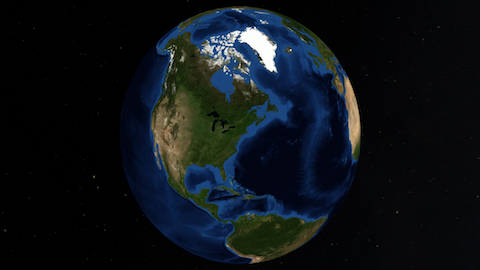
\includegraphics[width=\textwidth]{figures/results/os_view_earth.png}
        \caption{Earth}
    \end{subfigure}
    ~
    \begin{subfigure}[bt]{0.31\textwidth}
        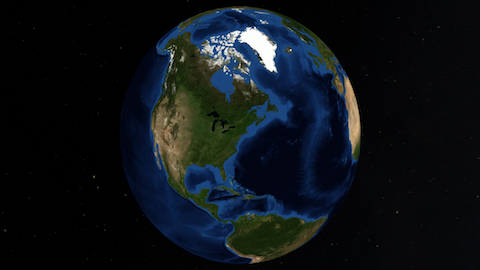
\includegraphics[width=\textwidth]{figures/results/os_view_earth.png}
        \caption{New York State}
    \end{subfigure}
    ~
    \begin{subfigure}[bt]{0.31\textwidth}
        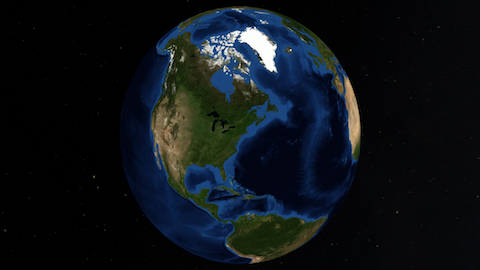
\includegraphics[width=\textwidth]{figures/results/os_view_earth.png}
        \caption{New York City}
    \end{subfigure}
    ~
    \begin{subfigure}[bt]{0.31\textwidth}
        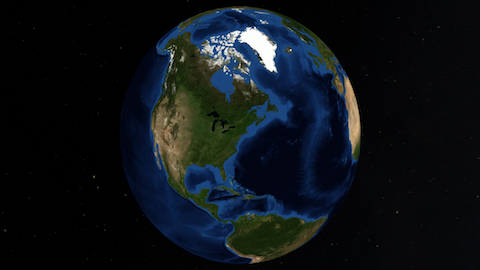
\includegraphics[width=\textwidth]{figures/results/os_view_earth.png}
        \caption{Manhattan}
    \end{subfigure}
    ~
    \begin{subfigure}[bt]{0.31\textwidth}
        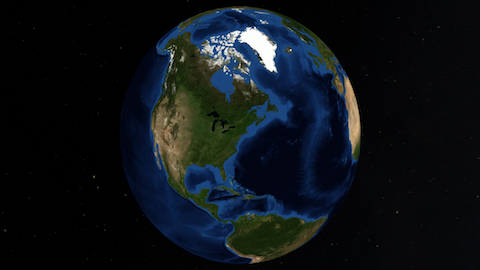
\includegraphics[width=\textwidth]{figures/results/os_view_earth.png}
        \caption{Central Park West}
    \end{subfigure}
    \caption{Top-down views of Earth at different zoom levels}
    \label{fig:topdown}
\end{figure}


\begin{table}
\centering
\caption[]{Top down settings}
  \label{table:settingstopdown}
  \begin{tabular}{| r | c c c c c |}
    \hline
      \textbf{Figure \ref{fig:topdown}}  & \textbf{a)} & \textbf{b)} & \textbf{c)} & \textbf{d)}  & \textbf{e)}  \\ \hline
      \textbf{Chunk Nodes}  & 10 & 54 & 66 & 102 & 106 \\ 
      \textbf{Leaf Chunk nodes} & 8 & 41 & 50 & 77 & 80 \\ 
      \textbf{Rendered Chunks} & 7 & 15 & 8 & 14 & 6 \\
      \textbf{Avg. FPS} & 48 & 42 & 42 & 40 & 41\\
    \hline
  \end{tabular}
\end{table}



\section{Benchmark: Horizontal view}
text here

\subsection{Culling for Distance based LOD}
text here

\subsection{Culling for Projected Area based LOD}
text here

\section{Benchmark: Interactive Globe Browsing}
text here

\section{Switching using level blending}
The visual result of using the distance based level blending is shown in Figure \ref{fig:blending2}.
\begin{figure}[htbp]
    \centering
    \begin{subfigure}[bt]{0.48\textwidth}
        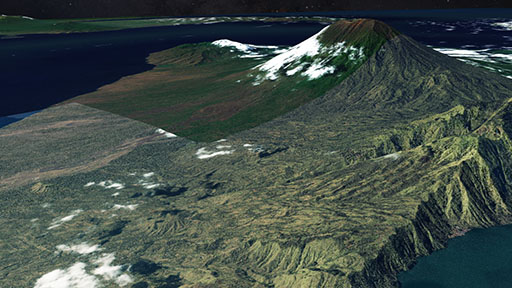
\includegraphics[width=\textwidth]{figures/results/blending/blending_bali2_disabled.jpg}
        \caption{No blending}
    \end{subfigure}
    \begin{subfigure}[bt]{0.48\textwidth}
        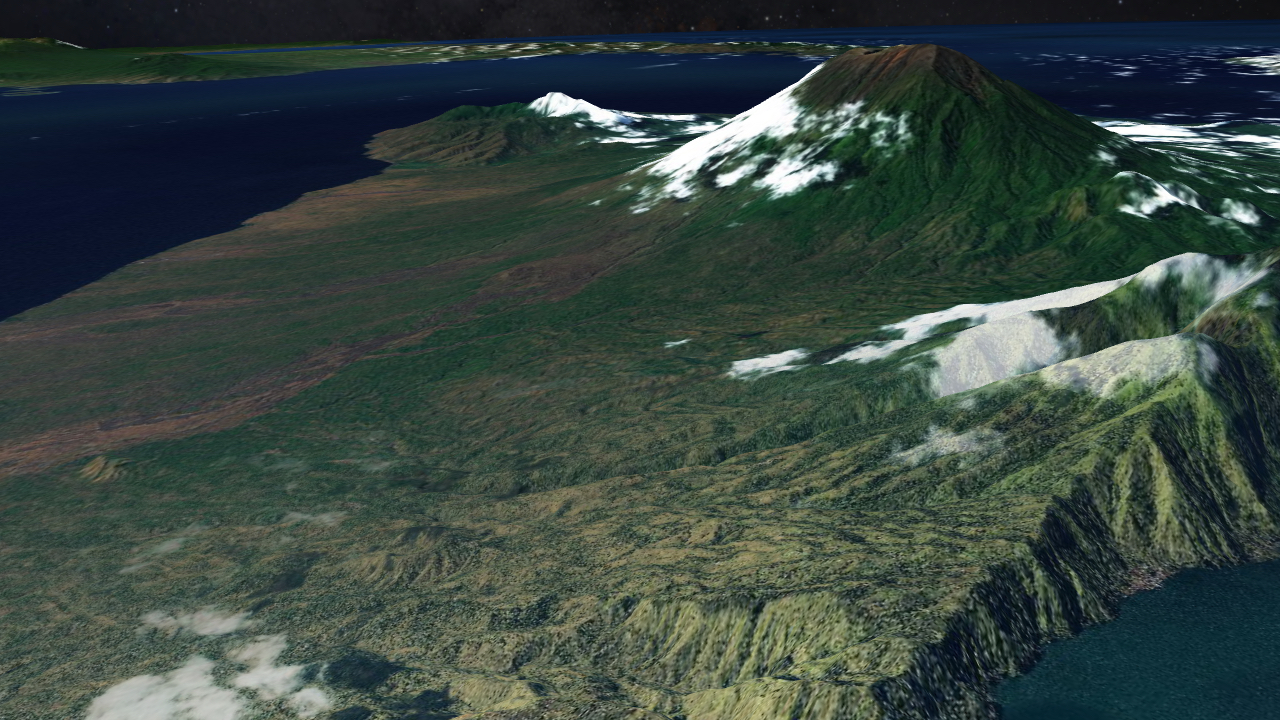
\includegraphics[width=\textwidth]{figures/results/blending/blending_bali2_enabled.jpg}
        \caption{Distance based level blending}
    \end{subfigure}
    \caption{Comparison of level blending and no blending. The LOD scale factor is set low to show the resolution penalty of using blending.}
    \label{fig:blending2}
\end{figure}


A performance benchmark of the blending algorithm is described below. Note that the in order to see the pixel resolution penalty of using level blending with the bear eye, the LOD scale factor was tuned down enough 

\begin{table}
  \centering
  \caption[]{Benchmark: Level blending}
    \label{table:settingstopdown}
  \begin{tabular}{| r l |}
    \hline
      \textbf{Globe:}             & Earth \\
      \textbf{Map datasets:}      & HeightLayers=[GCS\_Elevation\footnote{http://services.arcgisonline.com/ArcGIS/rest/services/ESRI\_Imagery\_World\_2D/MapServer}] \\
                                  & ColorLayers=[ESRI\_World\_2D\footnote{http://198.102.45.23/arcgis/rest/services/worldelevation3d/terrain3d?}] \\
      \textbf{LOD Scale factor:}  & 4.65 \\
      \textbf{LOD Evaluation:}    & By distance \\
      \textbf{Culling:}           & Frustum culling, Horizon culling \\
      \textbf{Camera View:}       & Horizon \\
    \hline
  \end{tabular}
\end{table}

\begin{figure}[htbp]
    \centering
    \begin{subfigure}[bt]{0.48\textwidth}
        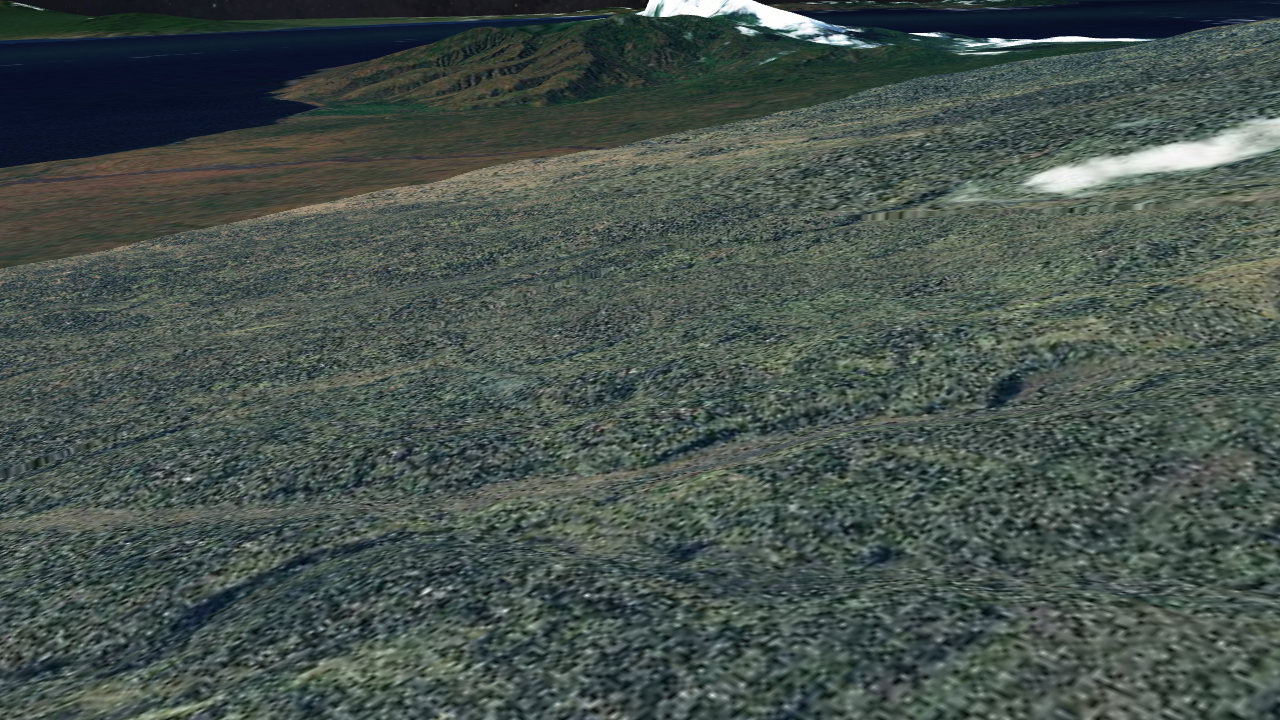
\includegraphics[width=\textwidth]{figures/results/blending/blending_bali_disabled.jpg}
        \caption{No blending}
    \end{subfigure}
    \begin{subfigure}[bt]{0.48\textwidth}
        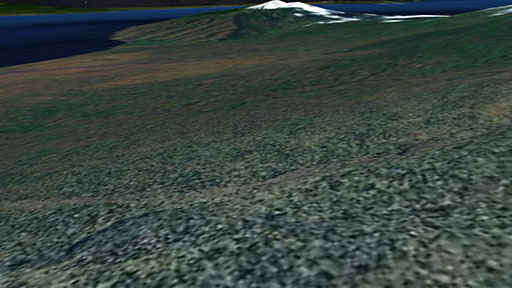
\includegraphics[width=\textwidth]{figures/results/blending/blending_bali_enabled.jpg}
        \caption{Level blending}
    \end{subfigure}
    \caption{Comparison of level blending and no blending. The LOD scale factor is set low to show the resolution penalty of using blending.}
    \label{fig:blending}
\end{figure}

\begin{table}
\centering
\caption[]{Top down settings}
  \label{table:settingstopdown}
  \begin{tabular}{| r | c c |}
    \hline
      \textbf{Figure \ref{fig:blending}}  & \textbf{No blending} & \textbf{Level blending} \\ \hline
      \textbf{Samples per fragment} & 1 & 3 \\ 
      \textbf{Avg. globe render time}  & 10.3 ms & 10.1 ms \\ 
      \textbf{Avg. frame time}  & 40 ms &  49 ms \\ 
      \textbf{Screenshot jpg size} & 1,1 MB & 0,7 MB \\
    \hline
  \end{tabular}
\end{table}



\section{Screenshots}
